\chapter{Task Planning}

\section{Introduction}
\label{sec:Introduction}


Task planning is a comprehensive strategy that instructs a robot on how to execute specific tasks to fulfill its primary goal. For robots such as Fire-Bots, which are designed for fire detection and suppression, task planning is crucial. It involves not only the identification and execution of tasks but also the optimal sequencing and timing of these actions. This is particularly vital in emergency situations where adaptability to dynamic environments is required.
In such complex and evolving scenarios, a hybrid task planner is typically employed. This approach integrates two principal components:

\textbf{1. Task Decomposition}: 
This involves breaking down complex tasks into simpler, manageable sub-tasks that the robot can execute efficiently. For Fire-Bots, this could involve segmenting a fire containment strategy into stages such as approach, assess, contain, and extinguish.

\textbf{2. Task Allocation}: 
This focuses on assigning these decomposed tasks to the robot or a fleet of robots, based on their capabilities, location, and the urgency of the tasks. In the context of our Fire-Bot, task allocation prioritizes fire detection and suppression while managing critical resources like battery life and water supply.

The hybrid task planner for the Fire-Bot, as discussed previously, operates within a system that merges hierarchical decision-making with reactive controls. It enables the robot to execute pre-planned actions for routine surveillance while remaining primed to react spontaneously to fire detection's or low battery alerts. This dual-layered strategy ensures that the Fire-Bot responds effectively to emergencies, maintaining a balance between its surveillance duties and its vital role in fire detection and extinguishing.



\section{Approach}
\label{sec:Approach}

In this part, we'll talk about how our Hybrid Planner works, which we introduced in section 3.1. Our method uses a mix of a step-by-step (Hierarchical) plan and an on-the-spot (Reactive) plan. This setup is designed to quickly adapt to changes while the robot is on fire watch duty, as shown in Figure 1

\label{sec:Approach}
\begin{figure}[h]
  \centering
  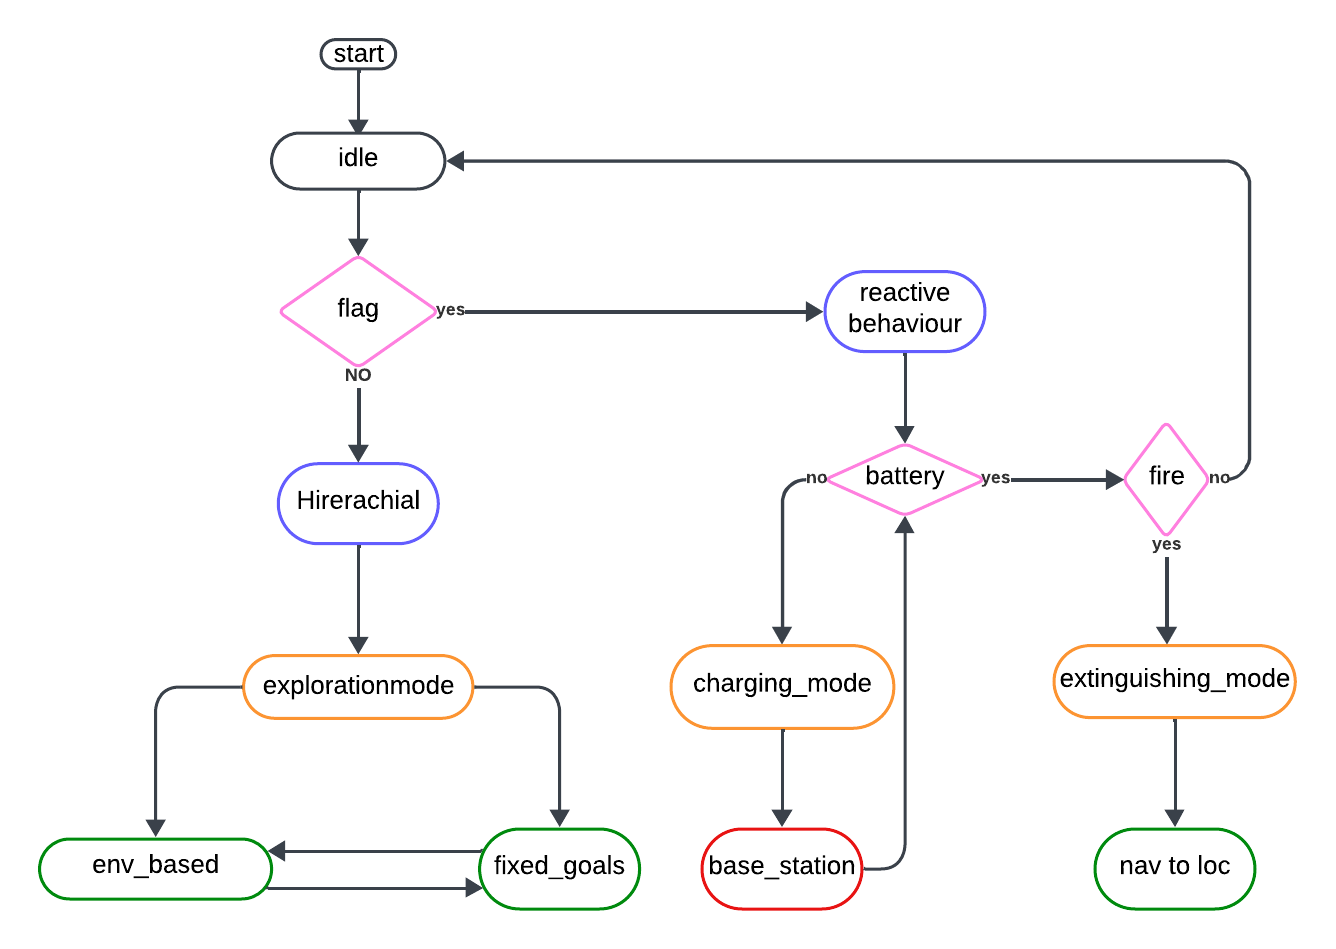
\includegraphics[width=0.9\textwidth, height=0.5\textheight]{Bilder/flow_chart.png}
  \caption{Flow chart for Hybrid Planner}
  \label{fig:flowchart}
\end{figure}

We break down the main goal into smaller tasks called Modes, such as Surveillance Mode for regular patrolling, Charging Mode for recharging the battery, and Extinguishing Mode for putting out fires. The planner can switch between these modes based on what's happening with the robot and any alerts it might get.

So, if the robot is going around checking for fires and suddenly finds one, it can switch to Extinguishing Mode to deal with the fire right away. Also, if the battery starts running low, the robot knows to switch to Charging Mode and navigate to base station to power up again. This way, Hybrid planner helps the robot do its job effectively, handling both its regular patrolling and any emergencies that come up.

\section{Implementation}



\begin{figure}[H]
\begin{algorithm}[H]
\DontPrintSemicolon
\SetKwFunction{FMoveToGoal}{MoveToGoal}
\SetKwFunction{FStopRobot}{StopRobot}
\SetKwFunction{FHandleFireDetection}{HandleFireDetection}
\SetKwFunction{FHandleLowBattery}{HandleLowBattery}
\SetKwFunction{FExecuteFireExtinguishing}{ExecuteFireExtinguishing}
\SetKwFunction{FExecuteCharging}{ExecuteCharging}
\SetKwFunction{FSwitchToSurveillanceMode}{SwitchToSurveillanceMode}
\SetKwFunction{FExplore}{Explore}
\SetKwProg{Fn}{Function}{:}{}
\Fn{\FMoveToGoal{x, y}}{
    \KwData{Goal coordinates \( x, y \)}
    \KwResult{Moves the robot to the specified coordinates}
    Send goal to action server with coordinates \( x, y \)\;
    Set robot state to "moving\_to\_goal"\;
}
\Fn{\FStopRobot{}}{
    \KwResult{Stops the robot by canceling its current goal}
    Publish cancel message to action server\;
    Set robot state to "idle"\;
}
\Fn{\FHandleFireDetection{}}{
    \KwResult{Handles the robot's behavior when fire is detected}
    \If{robot state is "idle" and battery level $\geq$ 10}{
        \FExecuteFireExtinguishing{}\;
    }
}
\Fn{\FHandleLowBattery{}}{
    \KwResult{Handles the robot's behavior when battery is low}
    \If{robot state is not "charging"}{
        \FExecuteCharging{}\;
    }
}
\Fn{\FExecuteFireExtinguishing{}}{
    \FStopRobot{}\;
    Move to the location of the fire\;
}
\Fn{\FExecuteCharging{}}{
    \FStopRobot{}\;
    Move to the charging station\;
}
\Fn{\FSwitchToSurveillanceMode{}}{
    \KwResult{Switches the robot to surveillance mode if it is idle}
    \If{robot state is "idle"}{
        \FExplore{}\;
    }
}
\Fn{\FExplore{}}{
    \KwResult{Runs the surveillance algorithm and optimizes the surveillance path}
    Run Exploration and set goals\;
    Run WayPointOptimizer and get best path\;
    \For{each goal in best path}{
        \If{fire detected or battery level $<$ 10}{
            break\;
        }
        \FMoveToGoal{goal.x, goal.y}\;
        Wait until goal is reached or failed\;
    }
    \If{not fire detected and battery level $\geq$ 10}{
        \FSwitchToSurveillanceMode{}\;
    }
}
\caption{Robot Controller Functions}
\end{algorithm}
\end{figure}
